\chapter{From CP to OMT}
\label{cha:OMTcore}

This chapter will discuss the CP-to-OMT problem and the implementation of an interface achieving this task. This work represents an additional step with respect to the SAT-to-Ising problem, but it could provide benefit to it: a new class of problems could be fed to quantum annealers and pave the way for new directions. 

\section{The first interface: FZN2OMT}

The first tentative to implement a CP-to-OMT converter is represented by FZN2OMT, developed by Patrick Trentin at the University of Trento and heavily discussed in \cite{cp2omt}. The interface, written in Python, managed the majority of issues raised in chapter 2.5.1 and is capable of translating a good variety of MiniZinc/FlatZinc problems. The compiler was developed in order to test the performance of OptiMathSAT in solving CP problems, which was an unexplored field at that time. Results showed how OMT solvers are usually penalized by the absence of procedures for global constraints and the management of Pseudo-Boolean constraints with respect to MiniZinc, offering cues for further studies and improvements. \\
One of the main issues behind this solver is its dependence from MathSAT: as already stated, OptiMathSAT is built on top of the SMT solver and, since it is proprietary code, the code cannot be distributed as open-source code. This condition prevents other computer scientists to easily test the bridge between the two paradigms and slows down the search of OptiMathSAT critical points to fix. As a consequence, the first goal we decided to pose was the independence from the SMT solver and the release of the code under the GNU General Public License v. 3.0 \cite{GPL}. \\
Once accomplished this first essential task, it was interesting to extend this primitive interface introducing new updates, most of them generated by MathSAT and OptiMathSAT evolution in the last years. Some arithmetics are currently not considered in the translation, in particular the Bit-Vector algebra (when expressly stated, Bit Vector variable are simply translated into SMT Integer variables); enabling it would improve the bridging between the two paradigms, speeding up the development of OMT.

\section{Open-source FZN2OMT}

In the next paragraphs we will discuss the workflow and the design choices adopted to build the open-source version of FZN2OMT. The first part will cover the development of an equivalent version of the previous FZN2OMT free from MathSAT dependencies, while improvements and extensions to the original tool will be discussed in the second section.

\subsection{Designing the skeleton}

In order to develop a standalone version of the interface satisfying the requirements underlined in paragraph 3.1, it was necessary to modify the majority of data structures and algorithms. The goal was to remove, when possible, procedures and structures which were useless for the tasks we wanted to integrate; the remaining cases required huge modifies to simplify their behaviour and step away from their original encoding. Lastly, all dependencies from the SMT solver had to be removed to avoid legal issues. \\
As a first step, we took the OptiMathSAT code and manually analyzed its structure to define the MathSAT dependencies that were useless for the paradigm conversion task. In particular, all references to algorithms dealing with the search of a valid solution were outside the scope of the project and promptly removed. Not all MathSAT libraries could be entirely removed from the project without impacting the execution of the code: the OMT and the SMT solvers share some data structures essential to efficiently build an SMT-LIB encoding. To ensure the possibility to license the new tool under GPL, all these structures and the methods calling them had to be re-written from scratches. In the beginning we were simply interested in making sure no link with the SMT solver were present in the final release: as a result, we built dummy classes with attributes and empty methods inspired by MathSAT files. \\
At the end of this process, we obtained an executable interface with no dependency from the SMT solver developed by UniTN and capable of scanning the input file, even though no translation is returned.
It is important to point out how the FlatZinc language parser was part of OptiMathSAT source code and it was not required to rewrite it nor modify its code.

\subsection{Storing variables and constants}

The skeleton built in chapter 7.2.1 represents the starting point to define a working interface, satisfying the requirements previously described and accepting all the FlatZinc problems managed by the old compiler. \\
The first aspect we concentrated on was the definition of classes for variables declared in the FlatZinc Language file. Since each variable can be associated to different data types, we first added a class to efficiently store information about the type, \textbf{DataType}; this information will help us in further manipulations and simplifications, as we will deepen later. A DataType is simply defined by a unique identifier and the name we assign to the represented type, such as Int or Real. Since the solvers do not admit user-defined types, we added an initialization procedure to create the relevant data types before we parse the CP file. \\
The next step was the definition of a class to store information about frequently used symbols, such as equality and addition; we named this class \textbf{Symbol}. This class does not differ too much the previous class: in addition to the name and the identifier we also associate its type using an instance of the DataType class.\\
Each variable is embedded in a class representing the basic unit of a formula, called \textbf{Term}. For the sake of simplicity, we designed this class reducing to the bone its body:

\begin{itemize}
    \item To identify and distinguish variables, we use the already mentioned combination of ID + name.
    \item To store its type we declare a Symbol with name identical to the one provided for the variable, that will also store the type thanks to its DataType attribute.
    \item Lastly, we introduced a vector of Term called \textit{children}. When creating variables, this attribute remains empty. Its importance will be cleared when discussing the creation of constraints.
\end{itemize}

The definition of constants is identical to the procedure for decision variables, with an additional step to link the symbol with its value. This association was managed creating an unordered map using the name as key and the assigned parameter as value. \\
All these newly created instances were collected defining a container class, \textbf{TermManager}.
A brief graph summing up the hierarchy of classes and their role in the program is shown in figure 7.1. 

\begin{figure}
    \centering
    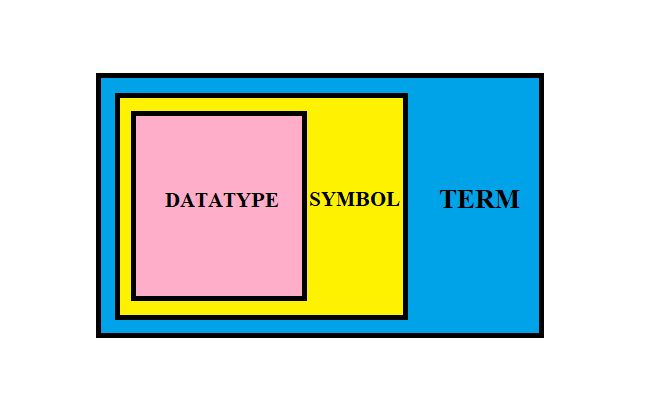
\includegraphics[width=0.75\textwidth]{images/hierarchy.png}
    \caption{An abstract representation of the class hierarchy in the open-source FZN2OMT interface.}
    \label{fig:my_label}
\end{figure}

\subsection{Introducing basic behaviour}

The fundamental task that the interface is required to satisfy is the encoding of FlatZinc constraints into SMT-LIB equivalent assertions. Some of these constraints (the MiniZinc manual calls them \textbf{FlatZinc builtins}) define simple relations among variables; the other constraints, \textit{global constraints}, represent high-level modelling abstractions, for which many solvers implement special, efficient inference algorithms and require more complex encoding. Each constraint is managed thanks to the introduction of a dedicate function. When all required arguments are constants, then it is quicker to evaluate the constraint using C datatypes and return as answer a SMT-LIB Bool variable. This is particularly useful when testing the correctness of the constraints and the parsing of the input file. Another special case happens when every arguments but the output decision variable are constant: in that case we , returning a nee Term whose type is linked to the input variables. As a general rule, if all variables are Integer, then we can create an Integer variables; on the other cases we choose Float in order not to lose precision nor information. This approach slightly reduces the amount of Boolean variables used and speed up the search of a valid solution. \\
In the remaining cases we translate the constraint into an assertion which will bind the value of the variables.

\subsection{Extending FZN2OMT}

Once the essential behaviours were implemented, we decided to extend the project adding that would increase its popularity and its usage.\\
First of all, OptiMathSAT is only one of the list of the OMT solvers available to the final users. Other popular solvers are z3 \cite{pa17} and Barcelogic \cite{barcelogic}, each one with their strengths and weaknesses. All these solvers support the SMT-LIB standard, but the format accepted by each tool presents some minor differences with respect to the others. Even though the community is currently working in removing these differences and provide a unified format to simply test a single instance of a problem in multiple tools, at the moment we need to adapt the SMT-LIB encoding to satisfy the semantic of each solver. Some of the most evident differences involve:

\begin{itemize}
    \item The setting of the background theory to exploit for a problem: since the SMT-LIB admits, for each tool we have to make sure a supported logic is passed, otherwise an error will be returned an the execution aborted. 
    \item The definition of the objective functions: each solver has different format to define the direction of the optimization and the cost function we are interested in optimizing.
\end{itemize}

Once read the manual guide for all these solvers and uniquely determined the differences that would cause an error, the best strategy that emerged to accomplish the task was the update of the \textit{Environment} class. Every time the declaration of a variable or an assertion is needed, the class now checks if the output language is not the default one and, in case of a positive answer, the string is modified before being written in the output file. The principal modifies concerns changes of keywords and the definition of the cost functions. The choice of the output solver is done when executing FZN2OMT: a command-line parameter has been added where the user can change the default output solver (OptiMathSAT) with the other tools named at the beginning of this section. The \textit{TermManager} class read this parameters and set a flag, enabling the translation in run-time when required.\\
The second extension proposed to the interface involves the Bit-Vector arithmetic. At the current state, FZN2OMT does not provide support for Bit-Vector encoding and Integer value cannot be mapped to an equivalent finite-precision encoding. On the other hand, huge progresses has been made in the definition of algorithms to efficiently search solutions for this theory, so testing this arithmetic would be of interest for the field Optimization Modulo Theories. SMT-LIB defines a different syntax for Bit-Vector variables and operations: as a result, the original structure of the \textit{Term} class has been extended. A new field has been added, \textit{class\_term}, indicating the size of the variable required to store the specific Integer value. If the variable is a constant, then the parameter is set in order to use the minimum number of bits to represent the number, otherwise a default value is set (the default value is originally set to 25, but it can be manually modified at execution time). This field is essential, since SMT-LIB requires to add the size of the variable when declared. \\
Once renovated the class, it was necessary to extend the arithmetic operations to avoid run-time error. In particular, we had to be careful while adding or multiplying BitVectors, since the size of the resulting variable dynamically depends from the starting terms. As a result, a set of new operator has been implemented starting from the relevant operators from the Integer and Float domain. When two constant are passed as input, then the interface simply compute the result of the operation and create a new variable storing it. On the opposite, if at least one of the input is a decision variable, then we have to create an empty variable whose size is capable of store values in the worst possible case, avoiding any Integer overflow issues. The heuristic adopted was the following:

\begin{itemize}
    \item In the case of additions or subtractions of two variables, we get the higher size between the two BitVectors and increase this value to 1.
    \item In the case of multiplications, we get the higher size between the two BitVectors and double it.
    \item The remaining operations, such as two's or one's complement, simply set the size of the resulting answer as equal to the input size.
\end{itemize}

The last step was the update of local and global constraints, so that they could handle BitVectors when asked. For each constraint in which the BitVector arithmetic actually impact the definition of the assertion, a map between Integer and their equivalent BitVector operations is generated. A flag in the \textit{Environment} class tracks the choice of the user about the type of encoding to apply, quickly swapping between the two typologies of functions. \\
For each operation, both the unsigned and the signed version are coded, covering the full extent of the arithmetic.
To enable the BitVector conversion we rely on a command-line parameter, in a fashion similar to the multi-language option. 

\newpage
